% ****************************************************************************************************
% Chapter 5: Text, Embeddings, and ClinicalBERT
% ****************************************************************************************************

\chapter{Text, Embeddings, and ClinicalBERT}
\label{ch:embeddings}

In Chapter~\ref{ch:features} I described the sixty-five tabular features that form the structured input to my model. This chapter is about the other half of the input: the fifty features derived from the chief complaint text. These are produced by a pipeline that takes a short string written by a triage nurse, passes it through a transformer-based language model, reduces the output with Principal Component Analysis, and hands the resulting vector to the downstream classifier.

The pipeline is not complicated, but several of the decisions behind it deserve explanation. Why a transformer rather than simpler representations? Which transformer, given that dozens of them exist? Should it be fine-tuned or used as-is? How should its 768-dimensional output be reduced? Each of these questions has a defensible answer, and for each I have some experimental evidence supporting my choice, including a few results that surprised me.

\section{Why Text at All}

The chief complaint is the single most informative free-text field available at triage. It is what the nurse writes down after asking the patient the simple question: ``What brings you in today?'' A string like ``substernal chest pain radiating to left arm, onset 2h'' carries very different clinical signal than ``ear pain $\times$ 3 days.'' Both are short, often under ten words, and neither lends itself to conventional tabular encoding. No single column can capture the range of meanings a chief complaint can express.

\begin{notebox}[What Is a Transformer Embedding, Intuitively?]
A transformer embedding is a vector of numbers, in my case 768 of them, that represents the ``meaning'' of a piece of text. The numbers themselves are not individually interpretable: there is no single dimension that means ``severity'' or ``cardiac.'' But in combination, they place the text in a geometric space where semantically similar texts end up near each other. ``Chest pain'' and ``pain in the chest'' produce nearly identical vectors; ``chest pain'' and ``ankle sprain'' produce very different ones.

The model that produces these embeddings, usually a BERT-family neural network, was originally trained to predict masked words in a large corpus of text. In the process, it learned representations that capture syntactic, semantic, and (for clinical models) medical relationships. I do not re-train it from scratch; I use the representations it already produces, possibly fine-tuning them further on my specific task.
\end{notebox}

My goal in using a transformer embedding is to let the downstream classifier exploit this semantic structure without having to rediscover it from raw characters. The alternative, bag-of-words or TF-IDF features, is simpler and cheaper, and I include one such baseline in the benchmark below. But it cannot capture that ``MI'' and ``myocardial infarction'' refer to the same condition, or that ``SOB'' and ``shortness of breath'' are synonyms. A well-chosen transformer can.

\section{The Benchmark: Nine Models, Two Datasets}

Before committing to any particular embedding model, I ran a systematic benchmark. The question was simple: on my actual data, which models produce embeddings that best capture the clinical signal relevant to triage acuity?

I tested nine models (Table~\ref{tab:embedding-models}), spanning three rough categories. First, two baselines to establish the floor of performance: a random 384-dimensional projection (essentially noise) and a TF-IDF bag-of-words vectorisation reduced to 50 dimensions. Second, five general-purpose sentence embedding models, including well-known models like \texttt{all-MiniLM-L6-v2} \citep{reimers2019sentence}, \texttt{all-mpnet-base-v2}, \texttt{BGE-base}, and two variants from the E5 family \citep{wang2022e5}. Third, two clinical-domain transformers: Bio\_ClinicalBERT \citep{alsentzer2019clinicalbert}, pretrained on clinical notes from MIMIC-III, and PubMedBERT \citep{gu2021pubmedbert}, pretrained on biomedical research articles.

\begin{table}[htbp]
 \centering
 \caption[Embedding models tested in the benchmark]{The nine models tested in the embedding benchmark. Three categories: baselines (random projection, TF-IDF), general-purpose sentence transformers, and domain-specific clinical transformers. All were evaluated with frozen weights, before any fine-tuning.}
 \label{tab:embedding-models}
 \small
 \begin{tabular}{lllc}
 \toprule
 Model & Architecture & Dim & Domain \\
 \midrule
 Random & 384d Gaussian random projection & 384 &, \\
 TF-IDF + SVD & Bag-of-words $\to$ truncated SVD & 50 &, \\
 MiniLM-L6 & 6-layer distilled BERT & 384 & General \\
 E5-small & E5 contrastive sentence encoder & 384 & General \\
 MPNet & Masked and permuted language modelling & 768 & General \\
 BGE-base & Contrastive pretraining, English & 768 & General \\
 E5-base & E5 contrastive, larger variant & 768 & General \\
 Bio\_ClinicalBERT & BERT-base, pretrained on MIMIC-III notes & 768 & Clinical \\
 PubMedBERT & BERT-base, pretrained on PubMed abstracts & 768 & Biomedical \\
 \bottomrule
 \end{tabular}
\end{table}

For each model, I extracted embeddings on both the Kaggle synthetic competition data (as a sanity check) and a five-percent sample of MIMIC-IV-ED (20,905 visits). I then evaluated the embeddings using intrinsic metrics, measures of how well the embedding space captures the label structure, computed without training any downstream classifier. The primary metrics were:

\begin{itemize}
 \item \textbf{kNN label purity at $k=10$}: for each visit, what fraction of its ten nearest neighbours in embedding space share its ESI level. A fully informative embedding would give purity close to one; a random embedding gives purity close to the class prior.
 \item \textbf{Linear probe F1}: the macro F1 achieved by a minimal logistic regression trained on frozen embeddings with 5-fold cross-validation. This is the simplest possible supervised classifier, used as a probe of how linearly separable the embeddings are.
 \item \textbf{Silhouette score, Calinski--Harabasz, Davies--Bouldin}: three clustering quality measures that quantify how well embeddings of the same class cluster together relative to embeddings of different classes.
\end{itemize}

The results, focusing on kNN purity and linear probe F1, are shown in Table~\ref{tab:benchmark-results}.

\begin{table}[htbp]
 \centering
 \caption[Embedding benchmark results on MIMIC-IV-ED and Kaggle]{Intrinsic evaluation results on five-percent samples of each dataset. kNN@10 is the fraction of a visit's ten nearest neighbours in embedding space sharing its ESI label. Linear probe F1 is macro F1 of a 5-fold logistic regression on frozen embeddings. Bold marks the best value in each column. The gap between clinical and general-purpose models on MIMIC is smaller than I expected, most models cluster within a few percentage points. On the synthetic Kaggle data, by contrast, clinical models win decisively, reflecting the severity-keyword text leakage described in Chapter~\ref{ch:discovery}.}
 \label{tab:benchmark-results}
 \small
 \begin{tabular}{lcccc}
 \toprule
 & \multicolumn{2}{c}{MIMIC-IV-ED} & \multicolumn{2}{c}{Kaggle synthetic} \\
 \cmidrule(lr){2-3} \cmidrule(lr){4-5}
 Model & kNN@10 & Probe F1 & kNN@10 & Probe F1 \\
 \midrule
 Random 384d & 0.412 & 0.162 & 0.261 & 0.191 \\
 TF-IDF + SVD50 & 0.546 & 0.270 & 0.549 & 0.486 \\
 MiniLM-L6 & 0.559 & 0.345 & \textbf{0.873} & 0.750 \\
 E5-small & 0.555 & 0.308 & 0.844 & 0.607 \\
 MPNet & 0.562 & 0.351 & 0.873 & 0.740 \\
 BGE-base & \textbf{0.566} & 0.330 & 0.867 & 0.687 \\
 E5-base & 0.565 & 0.317 & 0.852 & 0.629 \\
 Bio\_ClinicalBERT & 0.558 & 0.394 & 0.776 & \textbf{0.940} \\
 PubMedBERT & 0.558 & \textbf{0.399} & 0.649 & 0.883 \\
 \bottomrule
 \end{tabular}
\end{table}

\section{What the Benchmark Told Me}

The MIMIC results came as a partial surprise. I had expected the clinical-domain models, Bio\_ClinicalBERT and PubMedBERT, pretrained on medical text, to dominate the general-purpose models by a clear margin. They did not. On kNN purity at $k=10$, nearly all non-baseline models clustered within a two-percentage-point band ($0.546$ to $0.566$), with BGE-base actually leading. On linear probe F1, the clinical models did show an advantage ($0.394$--$0.399$ versus $0.308$--$0.351$ for the general-purpose models), but the gap was far smaller than the conventional wisdom around domain-specific pretraining would predict.

This is worth dwelling on. One common narrative in clinical NLP is that clinical-domain pretraining is transformative for clinical tasks: if you are working with medical text, you should always use a clinical model. My benchmark suggests a more measured claim: on frozen embeddings alone, clinical pretraining provides a modest advantage on linear probes, no advantage on kNN proximity, and is essentially tied with well-trained general-purpose sentence encoders. The structural information in a chief complaint like ``chest pain'' or ``shortness of breath'' is captured reasonably well by any competent transformer.

The Kaggle results, by contrast, are striking. On the synthetic competition data, Bio\_ClinicalBERT's linear probe F1 reaches 0.940, far above any other model. This is not a sign that ClinicalBERT understands the clinical content better. It is a sign that the Kaggle data contains the severity-keyword text leakage I documented in Chapter~\ref{ch:discovery}, and ClinicalBERT's vocabulary includes the severity adjectives (``severe,'' ``moderate,'' ``mild'') with enough structure that a linear classifier can exploit them. The gap between clinical and general models on Kaggle is a measure of text leakage, not of clinical signal. My own conclusion from this comparison was: frozen embeddings on MIMIC are roughly indistinguishable across models, and the text task as such has a ceiling around $0.40$ macro F1. To do better, I would need to fine-tune.

\begin{remarkbox}[A Lesson About Benchmarks]
When a benchmark produces a surprising result, the instinct is to check whether the benchmark is wrong. I spent some time on this, rerunning on a twenty-percent sample, verifying the metric implementations, checking for subtle bugs in preprocessing. The numbers held up. My initial expectation that clinical pretraining would dominate was simply incorrect for this task. This is the kind of finding that benchmarks are for: they discipline expectations that otherwise slip in unexamined.
\end{remarkbox}

\section{Fine-Tuning Bio\_ClinicalBERT}

Given that frozen embeddings plateau around $0.40$ F1, fine-tuning was the obvious next step. In fine-tuning, the pretrained model is trained further on a specific task, in my case, predicting the ESI acuity level from the chief complaint. Unlike frozen-embedding use, fine-tuning updates the model's internal weights, allowing the representation itself to specialise for the downstream task.

I chose Bio\_ClinicalBERT as the fine-tuning base, for three reasons. First, it tied PubMedBERT on the MIMIC benchmark while having lower parameter count and faster inference. Second, and more importantly, Bio\_ClinicalBERT was pretrained on MIMIC-III clinical notes, from the same institution (Beth Israel Deaconess Medical Center) that generated MIMIC-IV-ED. This is an unusually clean institutional match. The language, abbreviations, and documentation conventions that ClinicalBERT learned from MIMIC-III are essentially the same ones that appear in MIMIC-IV-ED triage notes. Third, it is the established standard in clinical NLP: much of the clinical ML literature since 2019 has used it as a baseline, which makes my results comparable to the existing body of work.

\begin{notebox}[Fine-Tuning versus Frozen Embeddings: What Is the Difference?]
When I use a pretrained model with frozen embeddings, I take its output for each input and feed that into my own classifier, but the pretrained model itself is unchanged. Its internal weights remain as they were after its original pretraining. I am using its general linguistic representations as they exist.

When I fine-tune, I attach a task-specific head (in my case, a linear layer mapping 768 dimensions down to 5 ESI class logits) and train the whole thing end-to-end on my labelled data. The weights deep inside the model move. The representation of ``chest pain'' after fine-tuning is no longer just a generic embedding of those two words, it is an embedding shaped by having seen, many times, which ESI labels are assigned to various chest-pain complaints in my training data.

Fine-tuning is more powerful but more expensive and more prone to overfitting. It also means the final embeddings are specific to this task and this dataset, rather than general-purpose. This is usually what you want, but it is a trade-off worth making deliberately.
\end{notebox}

\subsection*{Training Configuration}

My fine-tuning configuration is listed in Table~\ref{tab:finetune-config}. The values are standard for BERT-family fine-tuning tasks, with no exotic choices. Batch size 16 was the largest that fit in the sixteen-gigabyte VRAM of the T4 GPU along with FP16 mixed-precision training; a larger batch would not have changed the dynamics materially. Three epochs were sufficient; the best validation F1 was reached at epoch 2 in both my final configuration and in a separate lower-learning-rate sweep I discuss below. The linear warmup, standard for transformer fine-tuning, gradually increases the learning rate over the first ten percent of training to avoid early instability.

\begin{table}[htbp]
 \centering
 \caption[Bio\_ClinicalBERT fine-tuning configuration]{Fine-tuning hyperparameters for the final ClinicalBERT model. Values are standard for BERT-family fine-tuning. Best validation F1 was reached at epoch 2, consistent with the common finding that BERT models begin to overfit on small classification heads after two or three epochs of fine-tuning on a fixed dataset.}
 \label{tab:finetune-config}
 \small
 \begin{tabular}{ll}
 \toprule
 Hyperparameter & Value \\
 \midrule
 Base model & \texttt{emilyalsentzer/Bio\_ClinicalBERT} \\
 Optimizer & AdamW, weight decay 0.01 \\
 Learning rate & $2 \times 10^{-5}$ \\
 Learning rate schedule & Linear warmup (10\% of steps) then linear decay \\
 Batch size & 16 \\
 Max sequence length & 128 tokens \\
 Epochs & 3 \\
 Gradient clipping & Max norm 1.0 \\
 Dropout (classifier head) & 0.1 \\
 Mixed precision & FP16 (via \texttt{torch.amp.GradScaler}) \\
 Loss & Cross-entropy, unweighted \\
 Train / val / test split & 80 / 10 / 10 stratified \\
 Random seed & 42 \\
 Hardware & Standard\_NC4as\_T4\_v3 (T4 GPU, 16GB) \\
 Training time & 108 minutes (418{,}100 rows, 3 epochs) \\
 \bottomrule
 \end{tabular}
\end{table}

The classification head itself is minimal: a single linear layer mapping the 768-dimensional pooled representation to five logits, one per ESI class. I considered deeper heads (adding a hidden layer, or using a two-layer MLP) and did not pursue them. The general finding in BERT fine-tuning is that simple heads work best, the heavy lifting is done by the encoder's representations, and adding a complex head often hurts by introducing its own overfitting risk.

\subsection*{Pooling and Embedding Extraction}

After fine-tuning, I extract embeddings by running the fine-tuned encoder in inference mode on the full dataset. For each input, I take the encoder's final-layer hidden state, a 128-by-768 matrix, one 768-dimensional vector per token position, and compute a single 768-dimensional vector per visit by mean pooling over non-padding tokens. The classification head itself is discarded for this step; I am interested in the representation the encoder has learned, not in the classifier's five-dimensional output.

\begin{lstlisting}[language=Python, caption={The pooling and embedding extraction step. The classifier head is bypassed via \texttt{return\_embeddings=True}; only the mean-pooled encoder output is returned. Padding tokens are excluded from the mean via the attention mask.}]
def forward(self, input_ids, attention_mask, return_embeddings=False):
 outputs = self.encoder(input_ids=input_ids,
 attention_mask=attention_mask)
 pooled = self.mean_pool(outputs.last_hidden_state, attention_mask)
 if return_embeddings:
 return pooled # 768d, classifier head bypassed
 dropped = self.dropout(pooled)
 logits = self.classifier(dropped)
 return logits
\end{lstlisting}

I used mean pooling over non-padding tokens rather than the CLS-token representation (the first token in the sequence, which BERT-family models are sometimes trained to produce as a sequence-level summary). In the literature on sentence-transformer models, mean pooling has been reported to outperform CLS-token extraction for semantic similarity tasks when the model has not been specifically trained with a sentence-pair objective \citep{reimers2019sentence}. Bio\_ClinicalBERT was pretrained with masked language modelling rather than a sentence-level objective, so I expected mean pooling to be the safer default here. I did not run a head-to-head comparison of mean vs CLS pooling on this task; the choice was a sensible default rather than an experimentally-verified one.

The output is a single array of shape $418{,}100 \times 768$, containing one embedding per ED visit in my cohort. This array is saved to disk as a NumPy file and becomes the input to the next step: dimensionality reduction.

\subsection*{From 768 to 50: PCA Reduction}

Feeding 768-dimensional embeddings directly into a gradient-boosted decision tree is possible but inefficient. Tree models evaluate each feature independently at each split; high dimensionality inflates training time and memory use without proportional benefit when many dimensions encode redundant information. The standard solution is to reduce dimensionality via Principal Component Analysis (PCA).

\begin{notebox}[What Does PCA Do to an Embedding?]
Principal Component Analysis finds directions in the embedding space along which the data varies the most. The first principal component is the direction of maximum variance; the second is the direction of maximum remaining variance that is orthogonal to the first; and so on. Keeping the top 50 components (out of 768) preserves the directions in which the embeddings spread out the most, discarding directions where embeddings barely vary.

This is not lossless, I do lose some information. But for a classifier that benefits from most of its signal being in a low-dimensional subspace, PCA can speed up training substantially while barely affecting accuracy. In my case, the tradeoff is favourable: 50 PCA components capture enough of the embedding variance that the downstream F1 is indistinguishable from using 100 or 150 components.
\end{notebox}

I tested PCA dimensionalities of 50, 100, and 150. All three produced essentially identical downstream macro F1 of $0.541$ on the tabular-plus-text pipeline. I kept 50 as the default: there is no point paying for more dimensions if they do not improve performance. This PCA fitting is critical in one respect: I fit it \emph{within each cross-validation fold}, using only the training fold's embeddings, and then apply it to both training and validation embeddings for that fold. Fitting PCA globally, on the entire dataset before splitting, would introduce a subtle leak, since the principal directions would be informed by the validation data. I verified this was done correctly in the final pipeline; I had a variant earlier in development that did it incorrectly.

\section{Fine-Tuning Improved the Task, But Only Modestly}

The fine-tuned ClinicalBERT embeddings were the ones I used in the final blend pipeline. But it is worth being honest about how much the fine-tuning actually helped.

On the text-alone task, predicting ESI acuity from the chief complaint with no other features, fine-tuning raised macro F1 from the frozen ceiling of around $0.40$ to approximately $0.43$. This is a $+0.03$ improvement, real but modest. It does not transform the task. The text remains, on its own, a noisy signal for triage acuity on real data. Real nurses' chief complaints are terse, abbreviated, and sometimes cryptic (``pt c/o abd pain NOS''), and no amount of fine-tuning turns them into gold-standard labels.

Where the fine-tuned embeddings matter is in combination with tabular features. In the blend pipeline (Chapter~\ref{ch:architecture}), the fine-tuned text embeddings push the macro F1 from the honest-tabular-only baseline of approximately $0.56$ up to $0.597$. That is a more substantial $+0.04$ contribution. The text adds genuine signal that tabular features alone do not capture, the meaning of the chief complaint itself, above and beyond what vital signs and comorbidities reveal.

I also ran a systematic learning-rate sweep to check whether I was leaving performance on the table. A second run with learning rate $1 \times 10^{-5}$ and five epochs (instead of my default $2 \times 10^{-5}$ and three epochs) improved test F1 by $+0.003$, from $0.424$ to $0.427$. The best validation epoch in both configurations was epoch 2. I concluded that fine-tuning performance on this task is near its ceiling, given the data: longer training does not help, and a sweep over learning rates in the range commonly reported for BERT fine-tuning ($1$-$5 \times 10^{-5}$) yields differences within noise. This is a genuine limitation of the data rather than the training procedure.

\section{A Note About What SHAP Reveals}

Before closing this chapter, there is one finding from the fine-tuned embedding pipeline that I want to flag but defer to Chapter~\ref{ch:explainability} for full treatment.

When I run TreeSHAP analysis on the final blend model, the top features by importance are, almost without exception, embedding components. The first PCA component of the fine-tuned ClinicalBERT embedding (\texttt{emb\_pca\_0}) is the single most influential feature in the model, with a global SHAP magnitude roughly three times larger than any tabular feature. Three more embedding components follow in the top ten. The first clinically interpretable feature, NEWS2 score, appears further down the ranking.

This is not \emph{a priori} bad. A powerful text signal is exactly what fine-tuning is meant to produce. But it raises a concern: the model is making predictions that are heavily shaped by a numeric vector whose components have no human-readable interpretation. A clinician looking at the model's prediction cannot easily answer the question ``why did it say ESI-2?'' in terms of recognisable clinical reasoning.

More concerning still is what appears alongside the embedding components in the top feature list: \texttt{language} (the patient's primary language, used in interpretation services) and \texttt{insurance} (their insurance coverage) both rank in the top ten by SHAP magnitude. These are features that could plausibly encode social and demographic signal rather than clinical signal. The model may be learning to associate insurance type or language with acuity level in ways that reflect historical disparities in care rather than true clinical need. I return to this in Chapter~\ref{ch:fairness} with a full intersectional bias audit, and again in Chapter~\ref{ch:explainability} where I discuss what explainability requires and what the EU AI Act mandates.

\section{Dead Ends and What They Tell Me}

Three fine-tuning and embedding experiments did not work, and they are worth recording because each taught me something.

\paragraph{Dual embeddings: fine-tuned ClinicalBERT plus frozen MiniLM.} I hypothesised that combining my fine-tuned clinical embeddings with a frozen general-purpose embedding might capture complementary signal, general-world language structure that fine-tuning on clinical text might have partially overwritten. I concatenated MiniLM embeddings (384d, PCA-reduced to 50d) with the fine-tuned ClinicalBERT embeddings (768d, PCA-reduced to 50d) and retrained the full pipeline. The resulting F1 was 0.5558, versus 0.5556 for ClinicalBERT-only: a difference of two ten-thousandths, indistinguishable from noise. The lesson: fine-tuned clinical embeddings on my dataset already capture whatever general-purpose signal MiniLM contributed. Doubling the embedding dimensionality without adding new information is pure cost.

\paragraph{PCA dimensionality: 50, 100, 150.} I tested three PCA dimensions and got essentially identical results (F1 = 0.541 for all three). This confirms that the 50 principal components already capture the task-relevant variance. Higher-dimensional reductions add computation without benefit. I kept 50 as the default throughout the project.

\paragraph{Extended training: lower learning rate, more epochs.} The learning-rate sweep described above ($1 \times 10^{-5}$, five epochs) gained $+0.003$ F1. Given that the additional training time was roughly $2.5 \times$ the default (five epochs at lower learning rate converges more slowly), the marginal cost per unit improvement was high, and I did not adopt it as the default configuration. The finding I care about is not the specific number but the flatness of the learning-rate landscape: BERT fine-tuning is not particularly sensitive to precise hyperparameter choices within the common range, and obsessive hyperparameter tuning is rarely the largest lever for improvement.

\begin{figure}[htbp]
 \centering
 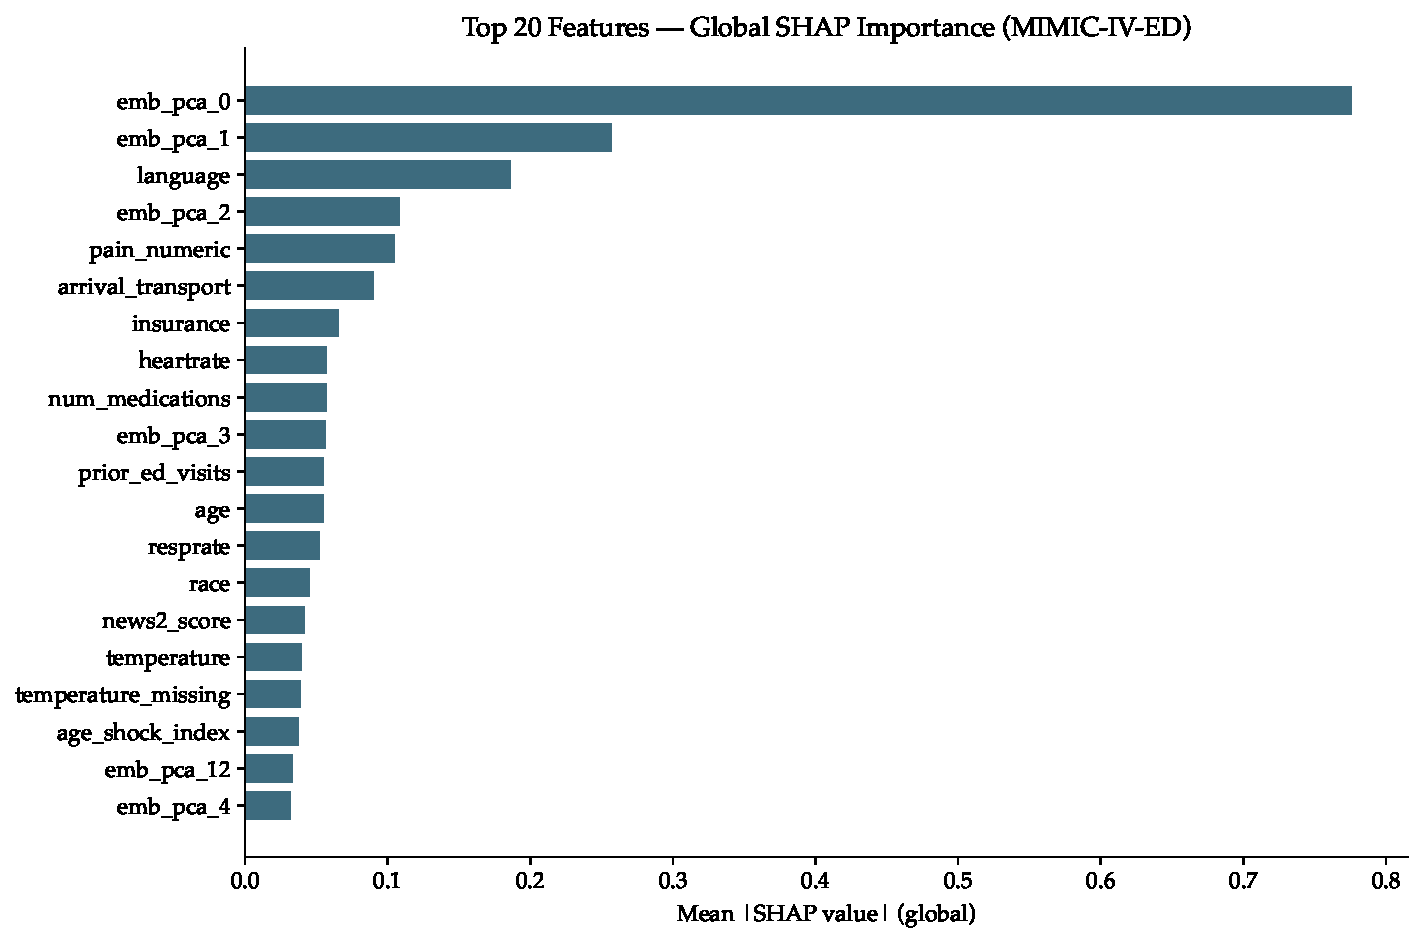
\includegraphics[width=0.9\textwidth]{figures/shap_bar_global.pdf}
 \caption[Global feature importance from TreeSHAP]{Mean absolute SHAP values for the top twenty features in the final blend model on MIMIC-IV-ED. The first principal component of the fine-tuned ClinicalBERT embedding (\texttt{emb\_pca\_0}) is more than twice as influential as any other feature. Three further embedding components appear in the top ten. Language and insurance, non-clinical demographic variables, also rank in the top ten. The first traditional clinical feature, NEWS2, does not appear until well down the list. I discuss the implications of this pattern, both positive and concerning, in Chapter~\ref{ch:explainability}.}
 \label{fig:shap-global-ch5}
\end{figure}

\begin{figure}[htbp]
 \centering
 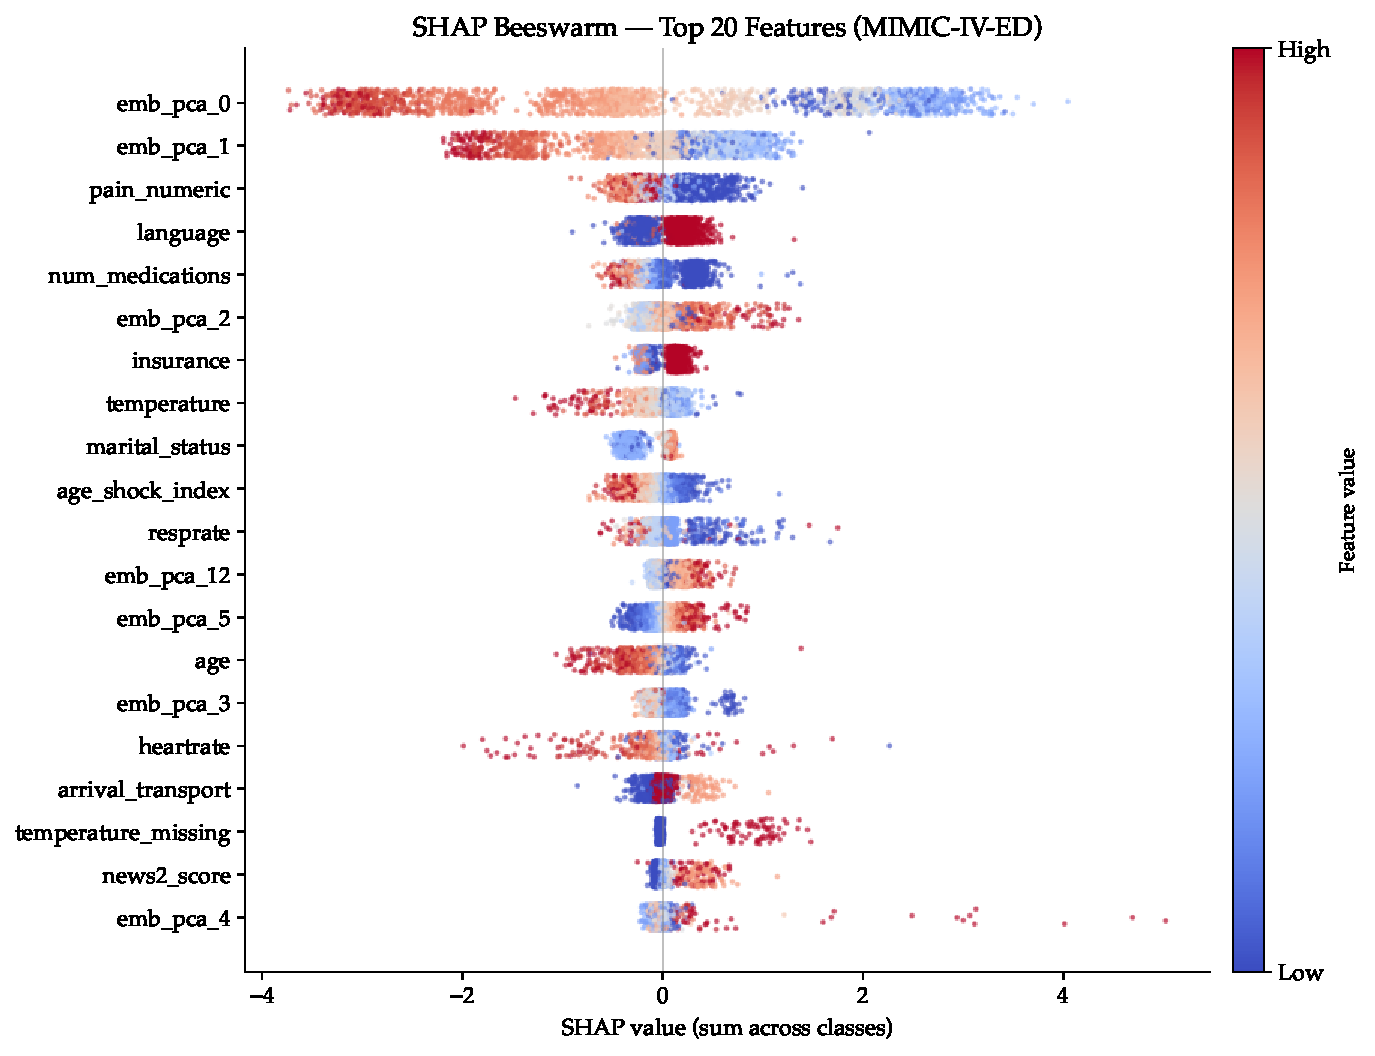
\includegraphics[width=0.9\textwidth]{figures/shap_beeswarm.pdf}
 \caption[SHAP beeswarm showing per-sample attributions]{SHAP beeswarm plot showing how individual features affect individual predictions across the dataset. Each dot is one patient. The horizontal spread indicates the magnitude and direction of the feature's contribution to that patient's predicted acuity; the colour indicates the feature's value (red high, blue low). The embedding components at the top of the chart dominate the plot, they pull predictions in both directions substantially more than most tabular features. This is the same pattern as the global summary but showing its per-patient texture.}
 \label{fig:shap-beeswarm-ch5}
\end{figure}

\section{What This Gives Me}

The text embedding pipeline, summarised: a fine-tuned Bio\_ClinicalBERT model produces a 768-dimensional vector for each chief complaint; PCA reduces this to 50 dimensions; the 50 components are concatenated with the 65 tabular features from Chapter~\ref{ch:features} to form the 115-dimensional input to the downstream classifier.

With this pipeline in hand, I can turn to the classifier itself. Chapter~\ref{ch:architecture} describes the model blend, the ensemble of gradient-boosted tree models, the stratified cross-validation scheme, the stacking meta-learner, and the threshold optimisation that produces the final prediction.
